\documentclass[letterpaper,11pt]{article}
\oddsidemargin -1.0cm \textwidth 17.5cm

\usepackage[utf8]{inputenc}
\usepackage[activeacute,spanish, es-lcroman]{babel}
\decimalpoint
\usepackage{amsfonts,setspace}
\usepackage{amsmath}
\usepackage{amssymb, amsmath, amsthm}
\usepackage{comment}
\usepackage{float}
\usepackage{amssymb}
\usepackage{dsfont}
\usepackage{anysize}
\usepackage{multicol}
\usepackage{enumerate}
\usepackage{graphicx}
\usepackage[left=1.5cm,top=1.5cm,right=1.5cm, bottom=1.7cm]{geometry}
\setlength\headheight{1.5em} 
\usepackage{fancyhdr}
\usepackage{multicol}
\usepackage{hyperref}
\usepackage{wrapfig}
\usepackage{subcaption}
\usepackage{siunitx}
\usepackage{cancel}
\pagestyle{fancy}
\fancyhf{}
\renewcommand{\labelenumi}{\normalsize\bfseries P\arabic{enumi}.}
\renewcommand{\labelenumii}{\normalsize\bfseries (\alph{enumii})}
\renewcommand{\labelenumiii}{\normalsize\bfseries \roman{enumiii})}

\begin{document}

\fancyhead[L]{\itshape{Facultad de Ciencias F\'isicas y Matem\'aticas}}
\fancyhead[R]{\itshape{Universidad de Chile}}

\begin{minipage}{11.5cm}
    \begin{flushleft}
        \hspace*{-0.6cm}\textbf{FI1100 Introducción a la Física Moderna}
    \end{flushleft}
\end{minipage}

\begin{picture}(2,3)
    \put(366, -10){
\includegraphics[scale=0.9]{Imágenes/logo/dfi-fcfm.pdf}}
\end{picture}

\begin{center}
	\LARGE\textbf{Problemitas de ondas}
\end{center}

\vspace{-1cm}

\begin{enumerate}\setlength{\itemsep}{0.4cm}

\rfoot[]{pág. \thepage}

\item[]

\item Se observa una onda que se transporta a lo largo de una cuerda, caracterizada por la ecuación:
$$y(x,t) = 4\sin{(2x-3t)}$$

\begin{enumerate}
    \item Verifique que esta función soluciona la ecuación de onda

    \item ¿En qué sentido se propaga la onda?

    \item Determine rapidez, longitud de onda y periodo

    \item ¿Cuál es la velocidad máxima de cualquier segmento de la cuerda?
\end{enumerate}

\item Una cuerda está dispuesta horizontalmente entre dos puntos separadas una distancia $L$. La cuerda tiene una densidad lineal $\rho$ y está tensada por una tensión $T$. Los extremos de la cuerda se hacen oscilar con una aceleración de la forma $a_0\sin{(\Omega t)}$ en sentido vertical, como se muestra en la figura. Se desea determinar la forma $y(x, t)$ de las ondas estacionarias formadas en la cuerda. Para esto, y considerando como solución inicial dos ondas sinusoidales que viajan en direcciones opuestas $y(x,t) = A\sin{(kx-\omega t)} + B\sin{(kx+\omega t)}$, siga los siguientes pasos:

\begin{enumerate}
    \item Escriba las condiciones de borde en los puntos $x=0$ y $x=L$

    \item Imponiendo las condiciones de borde, encuentre las relaciones entre: (i) $\Omega$ y $\omega$, (ii) $a_0$, $A$, $B$ y $\Omega$, (iii) $A$ y $B$

    \item Escriba, en forma compacta, la onda $y(x, t)$, y compare con la solución para ambos extremos fijos $y(x, t) = A\sin{(kx)}\cos{(\omega t)}$
\end{enumerate}

\begin{figure}[H]
    \centering
    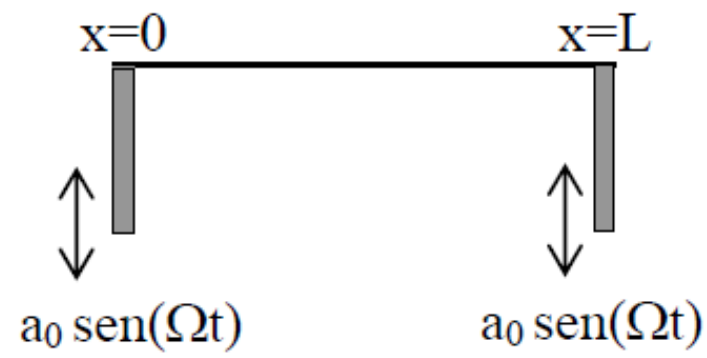
\includegraphics[width=0.4\linewidth]{Imágenes/clases/imagen_2023-08-30_151051968.png}
\end{figure}

\item Considere una cuerda de longitud $L$ y densidad de masa $\sigma$, bajo una tensión $\tau$, la cual está fija en un extremo y libre en el otro. Usando la superposición de dos ondas armónicas de igual amplitud que se propagan en sentido contrario, demuestre que la onda resultante es estacionaria, y que satisface las condiciones de borde respectivas. Además, demuestre que las frecuencias de los modos normales de este sistema cumplen la relación $f_n = (2n-1)/4L \cdot \sqrt{\tau/\sigma}$

\end{enumerate}
\end{document}